\documentclass[11pt, a4paper]{article}

\usepackage[T1]{fontenc}
\usepackage[utf8]{inputenc}
\usepackage[english]{babel} 
\usepackage{multicol}
\usepackage{lipsum}
\usepackage{ragged2e}
\usepackage{eurosym}
\usepackage{indentfirst}
\usepackage{titlesec}
\usepackage{pifont}
\usepackage{epsf}
\usepackage{booktabs}
\usepackage{multirow}
\usepackage{fancyhdr}
\usepackage[version=3]{mhchem}
\usepackage{color}
\usepackage{a4wide}
\usepackage{cite}
\usepackage{siunitx}
\usepackage{cmbright}

\addtolength{\voffset}{-1cm} % Top margin
\addtolength{\textheight}{2cm} % Bottom margin
\addtolength{\hoffset}{-1 cm} % Left margin 
\addtolength{\textwidth}{16 mm} % Right margin

%------- TXT --------
\usepackage{enumerate}
\usepackage[table,xcdraw]{xcolor}
%------- WEB --------
\usepackage{url}
\usepackage[colorlinks=true, allcolors=black]{hyperref}
%------- MATH --------
\usepackage{amsmath}
\usepackage{amsfonts}
\usepackage{amssymb}
%------- GRAPH -------
\usepackage{graphicx}
\usepackage{float}
\usepackage{wrapfig}
\usepackage{caption}
\usepackage{subcaption}
%------ CODE ---------
\usepackage{minted}

%To make an index:
\usepackage{imakeidx}
\makeindex[name=Tot,title={Index}]
\makeindex
% in the text : \index[Tot]{xxx}
% in the place where you want to put the index: \printindex[Tot]
% we can define a name other than "Tot" it's random, same for the index name we can put another title like {title= TFE Index}

% \addto\captionsenglish{\renewcommand{\chaptername}{Part}}

% --- Question box
\usepackage[most]{tcolorbox}
\tcbset{colback=gray!3, colframe=black!15, boxrule=0.3pt, arc=2mm, left=2mm, right=2mm, top=1mm, bottom=1mm}
\newtcolorbox{questionbox}{title=Question, fonttitle=\bfseries}


\graphicspath{ {./image/} }
\newcommand{\HRule}{\rule{\linewidth}{0.5mm}}

\begin{document}

\begin{titlepage}
    \begin{center}
        \vspace*{0.6cm}
    
        
\includegraphics[scale = 2.2]{uliege-hec.png}\\
        
        \vspace{1.5cm}
        
        % \textsc{\huge University of Liège}\\[1.2cm]
        
        \HRule \\[1cm]
        
        \textsc{\LARGE FINA0060-1: Empirical Methods in Financial Markets}\\[1cm]
        
        {\Huge \bfseries Final Assignment}\\[1.4cm] 
        
        \HRule \\[1cm]
    \end{center}
    
    \begin{minipage}{0.45\linewidth}
          \begin{flushleft} \large
          
            \emph{Group 1 : }\\
            Louis \textsc{HOGGE} s192814\\
            
          \end{flushleft}
    \end{minipage}
    \hfill
    \begin{minipage}{0.45\linewidth}
          \begin{flushright} \large
          
            \emph{Professor : } C. \textsc{HEUCHENNE}\\
            \emph{Year : } 2025-2026 
            
          \end{flushright}
    \end{minipage}
\end{titlepage}

\lhead{}
\rhead{}

\newpage

\pagenumbering{roman}

% \lhead{TABLE OF CONTENTS}
\tableofcontents

% %%%%%%%%%%%%%%%%%%%%%%%%%%%%%%%%%%%%%%%%%%%%%%%%%%%%%%%

\newpage

\pagenumbering{arabic}

\section{Trend} \label{trend_section}

\begin{questionbox}
    Why should we assume a trend? How could we characterize it?
\end{questionbox}

We adopt the additive decomposition
\[
    X_t \;=\; m_t \;+\; s_t \;+\; Y_t,
\]
where $m_t$ is the deterministic trend, $s_t$ a seasonal component, and $Y_t$ a (mean) stationary stochastic component.

\subsection{Why assume a trend?}
Visual inspection of $X_t$ against time reveals a systematic, smooth change in level across $t$ (Figure~\ref{fig:xt-over-time}) and a clear dependence of $X_t$ on $t$ in the scatter plot (Figure~\ref{fig:scatter-xt-t}). Such a pattern is consistent with a polynomial (nonlinear) trend rather than purely random fluctuations. 

\begin{figure}[H]
    \centering
    \begin{subfigure}[t]{.49\textwidth}
        
\includegraphics[width =\textwidth]{trend/step1a_Xt_over_time.png}
        \caption{$X_t$ over time.}
        \label{fig:xt-over-time}
    \end{subfigure}
    \hfill
    \begin{subfigure}[t]{.49\textwidth}
        
\includegraphics[width =\textwidth]{trend/step1a_scatter_Xt_vs_t.png}
        \caption{Scatter$(X_t,t)$.}
        \label{fig:scatter-xt-t}
    \end{subfigure}
    \caption{Visual inspection of $X_t$ against time.}
    \label{fig:visual_inspection_of_X_t_against_time}
\end{figure}

\subsection{How do we characterize it?}

\paragraph{Assumption.}
With the curvature observed in Figures~\ref{fig:xt-over-time}–\ref{fig:scatter-xt-t} we assume a deterministic cubic trend, i.e., $m_t$ is a time-invariant polynomial of degree three added to $X_t$. We thus estimate $X_t=\beta_0+\beta_1 t+\beta_2 t^2+\beta_3 t^3+\varepsilon_t$ by OLS, and the joint F-test is overwhelmingly significant, $F(3,2996)=2{,}530{,}484.246$, $p<10^{-16}$, with $R^2=0.9996$. All polynomial terms are individually significant, supporting a cubic deterministic trend. This suggests that up to three differences might in principle be required.

\paragraph{Actual differencing order determination.}
To follow the Box-Jenkins principle of using the smallest differencing order that makes the series approximately stationary in mean (to avoid over-differencing), we compute $\nabla^d X_t$ for $d\in\{1,2,3\}$ and regress each differenced series on a constant and a linear time trend. For $d=1$ the slope remains highly significant, so the trend is clearly not removed. 

\begin{figure}[H]
    \centering
    \begin{subfigure}[t]{.49\textwidth}
        
\includegraphics[width =\textwidth]{trend/step1d_diff1_series.png}
        \caption{First-order differenced series $\nabla^1 X_t$.}
        \label{fig:diff1}
    \end{subfigure}
    \hfill
    \begin{subfigure}[t]{.49\textwidth}
        
\includegraphics[width =\textwidth]{trend/step1d_diff1_scatter_with_OLS.png}
        \caption{Scatter$(\nabla^1 X_t, t)$ with OLS fit.}
        \label{fig:diff1-scatter-ols}
    \end{subfigure}
    \caption{First-order differencing diagnostics for $X_t$}
    \label{fig:first_order_differencing_diagnostics_for_X_t}
\end{figure}

For $d=2$ the slope is still statistically significant ($p=6.78\times 10^{-4}$) but the estimated coefficient is extremely small: over the entire sample ($\approx3000$ observations) the implied drift in $\nabla^2 X_t$ is less than $3$ units ($|\hat\beta| \times 3000 = 0.0009774 \times 3000 \approx 2.93$). In other words, the residual trend is negligible in practice and Figure~\ref{fig:second_order_differencing_diagnostics_for_X_t} shows no visible deterministic pattern.

\begin{figure}[H]
    \centering
    \begin{subfigure}[t]{.49\textwidth}
        
\includegraphics[width =\textwidth]{trend/step1d_diff2_series.png}
        \caption{Second-order differenced series $\nabla^2 X_t$.}
        \label{fig:diff2}
    \end{subfigure}
    \hfill
    \begin{subfigure}[t]{.49\textwidth}
        
\includegraphics[width =\textwidth]{trend/step1d_diff2_scatter_with_OLS.png}
        \caption{Scatter$(\nabla^2 X_t, t)$ with OLS fit.}
        \label{fig:diff2-scatter-ols}
    \end{subfigure}
    \caption{Second-order differencing diagnostics for $X_t$.}
    \label{fig:second_order_differencing_diagnostics_for_X_t}
\end{figure}

For $d=3$ the slope becomes statistically insignificant. However, in our setting the sample size is large, so formal t-tests are very sensitive and tend to reject even tiny departures from zero. Moreover, at this stage the sample SACF of $\nabla^d X_t$ remains very large for all d due to strong seasonal dependence. The SACF band test therefore does not discriminate between d values and seasonal non-stationarity is treated separately in Step 3.\\

Following the Box-Jenkins guideline, and given that the trend component is already effectively removed at $d=2$, we choose this order. A third difference would risk over-differencing without providing a meaningful improvement in the trend diagnostics.

\paragraph{Removing the polynomial trend.} 
We remove a polynomial trend of degree $d$ by differencing of order $d$ implemented with \texttt{lagmatrix}. Specifically, for $d=2$ we apply the second difference
\[
\nabla^2 X_t \;=\; X_t - 2 X_{t-1} + X_{t-2},
\]
This removes the dominant cubic trend component up to an approximately constant mean, providing a stationary-looking series in level for subsequent seasonal and ARMA modeling.

% \newpage

\section{Seasonality} \label{seasonality_section}

\begin{questionbox}
    Why should we assume a seasonal component? How could we characterize it?
\end{questionbox}

After removing the deterministic trend (Section~\ref{trend_section}), we inspect the autocorrelation of the detrended series $r_1(t)$ to assess seasonality. A seasonal pattern of period $S$ manifests as a sequence of pronounced SACF spikes at lags $S,\,2S,\,3S,\ldots$

\subsection{Why assume a seasonal component?}

The sample SACF of $r_1(t)$ (Figure~\ref{fig:acf-before-seasonal}) exhibits regularly spaced peaks that exceed the sampling bands, indicating serial dependence repeating at a fixed interval. This repeating structure is characteristic of a seasonal component rather than a one-off persistence effect.

\begin{figure}[H]
  \centering
  
\includegraphics[width=0.5\linewidth]{seasonality/step2a_acf_before_seasonal.png}
  \caption{Sample SACF of $r_1(t)$ before seasonal differencing.}
  \label{fig:acf-before-seasonal}
\end{figure}

\subsection{How do we characterize it?}

\paragraph{Assumption.}
We assume a seasonal period $S=4$ from the spacing between significant SACF peaks. 

% \paragraph{Formal seasonal period determination.}
% We validate the choice of $S$ using a \emph{seasonal-only} Ljung-Box test that targets multiples of $S$, $H_0(S):\ \rho(\ell)=0$ for $\ell\in\{S,2S,3S,\ldots\}$. For each $S\in\{2,\ldots,20\}$ we compute $Q_{\text{pre}}(S)$ on $r_1(t)$ and $Q_{\text{post}}(S)$ on $Y(t)=\nabla_S r_1(t)$, retain those with $p_{\text{pre}}(S)<0.05$ and $p_{\text{post}}(S)>0.05$, and among this set choose the value closest to the ACF-based guess $\hat S_{\text{ACF}}=4$. We obtain the post-differencing results in Table~\ref{tab:seasonal-lb-grid}. The non-rejected candidates are $S\in\{4,8,12,16,20\}$, and the smallest and closest candidate to the ACF-based guess is $S=4$ (all other candidates have $p_{\text{post}}$ numerically indistinguishable from zero).

% \begin{table}[H]
%     \centering
%     \begin{tabular}{lrrr}
%         \toprule
%         $S$ & $Q_{\text{post}}$ & $p_{\text{post}}$ & Decision ($\alpha=0.05$) \\
%         \midrule
%         4  & $6.340$ & $0.2745$ & Fail to reject \\
%         8  & $1.610$ & $0.4471$ & Fail to reject \\
%         12 & $2.354$ & $0.1250$ & Fail to reject \\
%         16 & $0.016$ & $0.8998$ & Fail to reject \\
%         20 & $2.200$ & $0.1380$ & Fail to reject \\
%         \bottomrule
%     \end{tabular}
%     \caption{Seasonal-only Ljung-Box across candidate $S$ (post-differencing)}
%     \label{tab:seasonal-lb-grid}
% \end{table}

\paragraph{Removing the seasonality.} 
We remove seasonality by applying the seasonal difference operator
\[
\nabla_{4} r_1(t) \;=\; r_1(t) - r_1(t-4),
\]
which yields the deseasonalized series $Y(t)=\nabla_{4} r_1(t)$ suitable for stationary modeling.

\begin{figure}[H]
    \centering
    \begin{subfigure}[t]{.49\textwidth}
        
\includegraphics[width =\textwidth]{seasonality/step2b_seasdiff_S4_series.png}
        \caption{Seasonally differenced series $Y(t)=\nabla_{4} r_1(t)$.}
        \label{fig:seasdiff-series}
    \end{subfigure}
    \hfill
    \begin{subfigure}[t]{.49\textwidth}
        
\includegraphics[width =\textwidth]{seasonality/step2b_seasdiff_S4_scatter_with_OLS.png}
        \caption{Scatter of $Y(t)=\nabla_{4} r_1(t)$ vs.\ $t$ with OLS fit.}
        \label{fig:seasdiff-scatter}
    \end{subfigure}
    \caption{Forth-order seasonal differencing diagnostics for $Y_t$.} 
    \label{fig:seasdiff-post}
\end{figure}

\paragraph{Check post-deseasonalization.}
After differencing with $S=4$, the seasonal spikes collapse and the SACF at multiples of $4$ lies within the $\pm 1.96/\sqrt{N}$ bands in Figure~\ref{fig:acf-after-seasonal}.

\begin{figure}[H]
  \centering
  
\includegraphics[width=0.5\linewidth]{seasonality/step2c_acf_after_seasonal_S4.png}
  \caption{SACF of $Y(t)=\nabla_{4} r_1(t)$ after seasonal differencing.}
  \label{fig:acf-after-seasonal}
\end{figure}

The seasonal-only portmanteau switches from strong rejection to non-rejection:
\[
\text{pre (on }r_1):\ Q=14700.194,\ \mathrm{df}=5,\ p<10^{-16};\qquad
\text{post (on }Y_t):\ Q=6.340,\ \mathrm{df}=5,\ p=0.2745.
\]

% \newpage

\section{Stationarity} \label{stationarity_section}

\begin{questionbox}
    What stationary model seems to be the best to model the behavior of Yt? Is a pure random process suitable? Are all the underlying hypotheses respected?
\end{questionbox}

After removing the deterministic trend and seasonality, we focus on the stochastic component $Y_t$, we analyze it and try to model it.

\subsection{Is a pure random process suitable for $Y_t$?}

\paragraph{Normality diagnostics.}
Let's first check if the marginal distribution of $Y_t$ is compatible with the usual Gaussian assumption. The histogram of $Y_t$ (Figure~\ref{fig:prelim-y-hist}) is roughly bell-shaped and symmetric, and the points in the QQ-plot (Figure~\ref{fig:prelim-y-qq}) lie close to the 45-degree line, with no clear systematic deviations in the tails. A Kolmogorov-Smirnov test against a normal distribution $N(\mu,\sigma)$, where $\mu$ ($=-0.00328$) and $\sigma$ ($=1.169$) are estimated by the sample mean and standard deviation of $Y_t$, yields a test statistic of $0.0125$ and a $p$-value of $0.7328$. Thus we do \emph{not} reject the Gaussian assumption for the marginal distribution of $Y_t$.

\begin{figure}[H]
  \centering
  \begin{subfigure}[t]{.49\textwidth}
    
\includegraphics[width=\textwidth]{stationarity/step3a_prelim_hist_Yt.png}
    \caption{Histogram of $Y_t$.}
    \label{fig:prelim-y-hist}
  \end{subfigure}\hfill
  \begin{subfigure}[t]{.49\textwidth}
    
\includegraphics[width=\textwidth]{stationarity/step3a_prelim_qqplot_Yt.png}
    \caption{QQ-plot (standardized $Y_t$ vs.\ $N(0,1)$).}
    \label{fig:prelim-y-qq}
  \end{subfigure}
  \caption{Normality checks for $Y_t$.}
  \label{fig:prelim-y-hist-qq}
\end{figure}

\paragraph{Sample autocorrelation function (SACF).}
Let's now check if $Y_t$ is i.i.d. The SACF of $Y_t$ obtained post-deseasonalization in the previous section (Section~\ref{seasonality_section}, Figure~\ref{fig:acf-after-seasonal}) exhibits a large negative spike at lag~1 (around $-0.4$), far outside the $\pm 1.96/\sqrt{N}$ band, while at higher lags the auto-correlations are much smaller and mostly lie within the band. This indicates strong negative short-run dependence and this behavior is inconsistent with i.i.d.\ white noise, for which all auto-correlations should be close to zero.

\paragraph{Ljung-Box test.}
To formalize the graphical SACF check, we perform Ljung-Box portmanteau tests for several values of the lag order $h$. All the $Q(h)$ statistics in table~\ref{tab:yt-ljungbox} are extremely large and the corresponding $p$-values are essentially zero, for all considered lags. Hence, the null hypothesis of no serial correlation up to lag $h$ is decisively rejected. 

\begin{table}[H]
  \centering
  \caption{Ljung-Box statistics for $Y_t$.}
  \label{tab:yt-ljungbox}
  \begin{tabular}{ccc}
    \hline
    Lag $h$ & $Q(h)$ & $p$-value \\
    \hline
     5  & 461.8 & $<10^{-16}$ \\
    10  & 470.5 & $<10^{-16}$ \\
    15  & 475.8 & $<10^{-16}$ \\
    20  & 476.8 & $<10^{-16}$ \\
    \hline
  \end{tabular}
\end{table}

Together with the SACF plot, this confirms that $Y_t$ cannot be modeled as a pure random process.

\paragraph{Stationarity check.}
Since we now know that a stationary ARMA-type model is required to capture the residual dependence structure of $Y_t$, let's run an augmented Dickey-Fuller test for a unit root. With a constant and zero lagged differences, the ADF statistic is $-82.39$ and the associated $p$-value is $0$, so the null hypothesis of a unit root is overwhelmingly rejected and we can treat $Y_t$ as a stationary process.

\subsection{What is the best stationary model for $Y_t$? Are hypotheses respected?}

\paragraph{Assumption.}
From Figure~\ref{fig:prelim-y-acf-pacf}, we observe that the SACF of $Y_t$ displays a large negative spike at lag~1, followed by additional negative spikes at lags~4 and~9, with subsequent lags being much smaller in magnitude. Meanwhile, the SPACF remains mostly negative and decays smoothly. Such a pattern is characteristic of a moving-average process with negative coefficients.

\begin{figure}[H]
  \centering
  \begin{subfigure}[t]{.49\textwidth}
    
\includegraphics[width=\textwidth]{stationarity/step3a_prelim_sacf_Yt.png}
    \caption{SACF of $Y_t$.}
  \end{subfigure}\hfill
  \begin{subfigure}[t]{.49\textwidth}
    
\includegraphics[width=\textwidth]{stationarity/step3a_prelim_spacf_Yt.png}
    \caption{SPACF of $Y_t$.}
  \end{subfigure}
  \caption{Dependence diagnostics for $Y_t$ (bands at $\pm 1.96/\sqrt{N}$).}
  \label{fig:prelim-y-acf-pacf}
\end{figure}

\paragraph{Model selection.}
We first test simple MA specifications guided by the significant SACF lags. Both an $\mathrm{MA}(1)$ model and a sparse $\mathrm{MA}(1,4,9)$ model yield residuals for which the Ljung-Box tests systematically fail to reject the null hypothesis of no remaining serial correlation.\\

To refine the model, we then incrementally expand the set of MA lags by incorporating the SACF-significant residual lags. Starting from $\mathrm{MA}(1)$, we test $\mathrm{MA}(1,3,4,5)$, for which the Ljung-Box tests still fail, and then $\mathrm{MA}(1,2,3,4,5)$, which passes all Ljung-Box tests. Likewise, starting from $\mathrm{MA}(1,4,9)$, we test $\mathrm{MA}(1,2,3,4,9)$, which also passes Ljung-Box tests.\\

Because these two models share a common subset of lags, we prune the less significant outer lags (5 and 9). The resulting $\mathrm{MA}(1,2,3,4)$ model keeps all essential dynamics while improving parsimony.   It satisfies the invertibility condition with the minimum modulus of the MA roots being equal to $1.1232 > 1$. It remains fully validated by Ljung-Box tests with statistics at lags 5 to 30 all producing $p$-values strictly above~0.11 and the SACF and SPACF of the residuals looking good (Figure~\ref{fig:prelim-y-acf-pacf}). Finally, it achieves the lowest BIC ($=0.0115$) among all candidate models.\\

\begin{figure}[H]
  \centering
  \begin{subfigure}[t]{.49\textwidth}
    
\includegraphics[width=\textwidth]{stationarity/step3c_resid_sacf_MA.png}
    \caption{SACF of $\mathrm{MA}(1,2,3,4)$ residuals.}
  \end{subfigure}\hfill
  \begin{subfigure}[t]{.49\textwidth}
    
\includegraphics[width=\textwidth]{stationarity/step3c_resid_spacf_MA.png}
    \caption{SPACF of $\mathrm{MA}(1,2,3,4)$ residuals.}
  \end{subfigure}
  \caption{Dependence diagnostics for $\mathrm{MA}(1,2,3,4)$ residuals.}
  \label{fig:yt-ma-resid-acf-pacf}
\end{figure}

Concerning normality, the histogram and QQ-plot of the residuals are still looking good. Moreover, the Kolmogorov-Smirnov test returns a statistic of $0.0088$ with $p=0.9751$, so the Gaussian assumption is still not rejected.

\begin{figure}[H]
  \centering
  \begin{subfigure}[t]{.49\textwidth}
    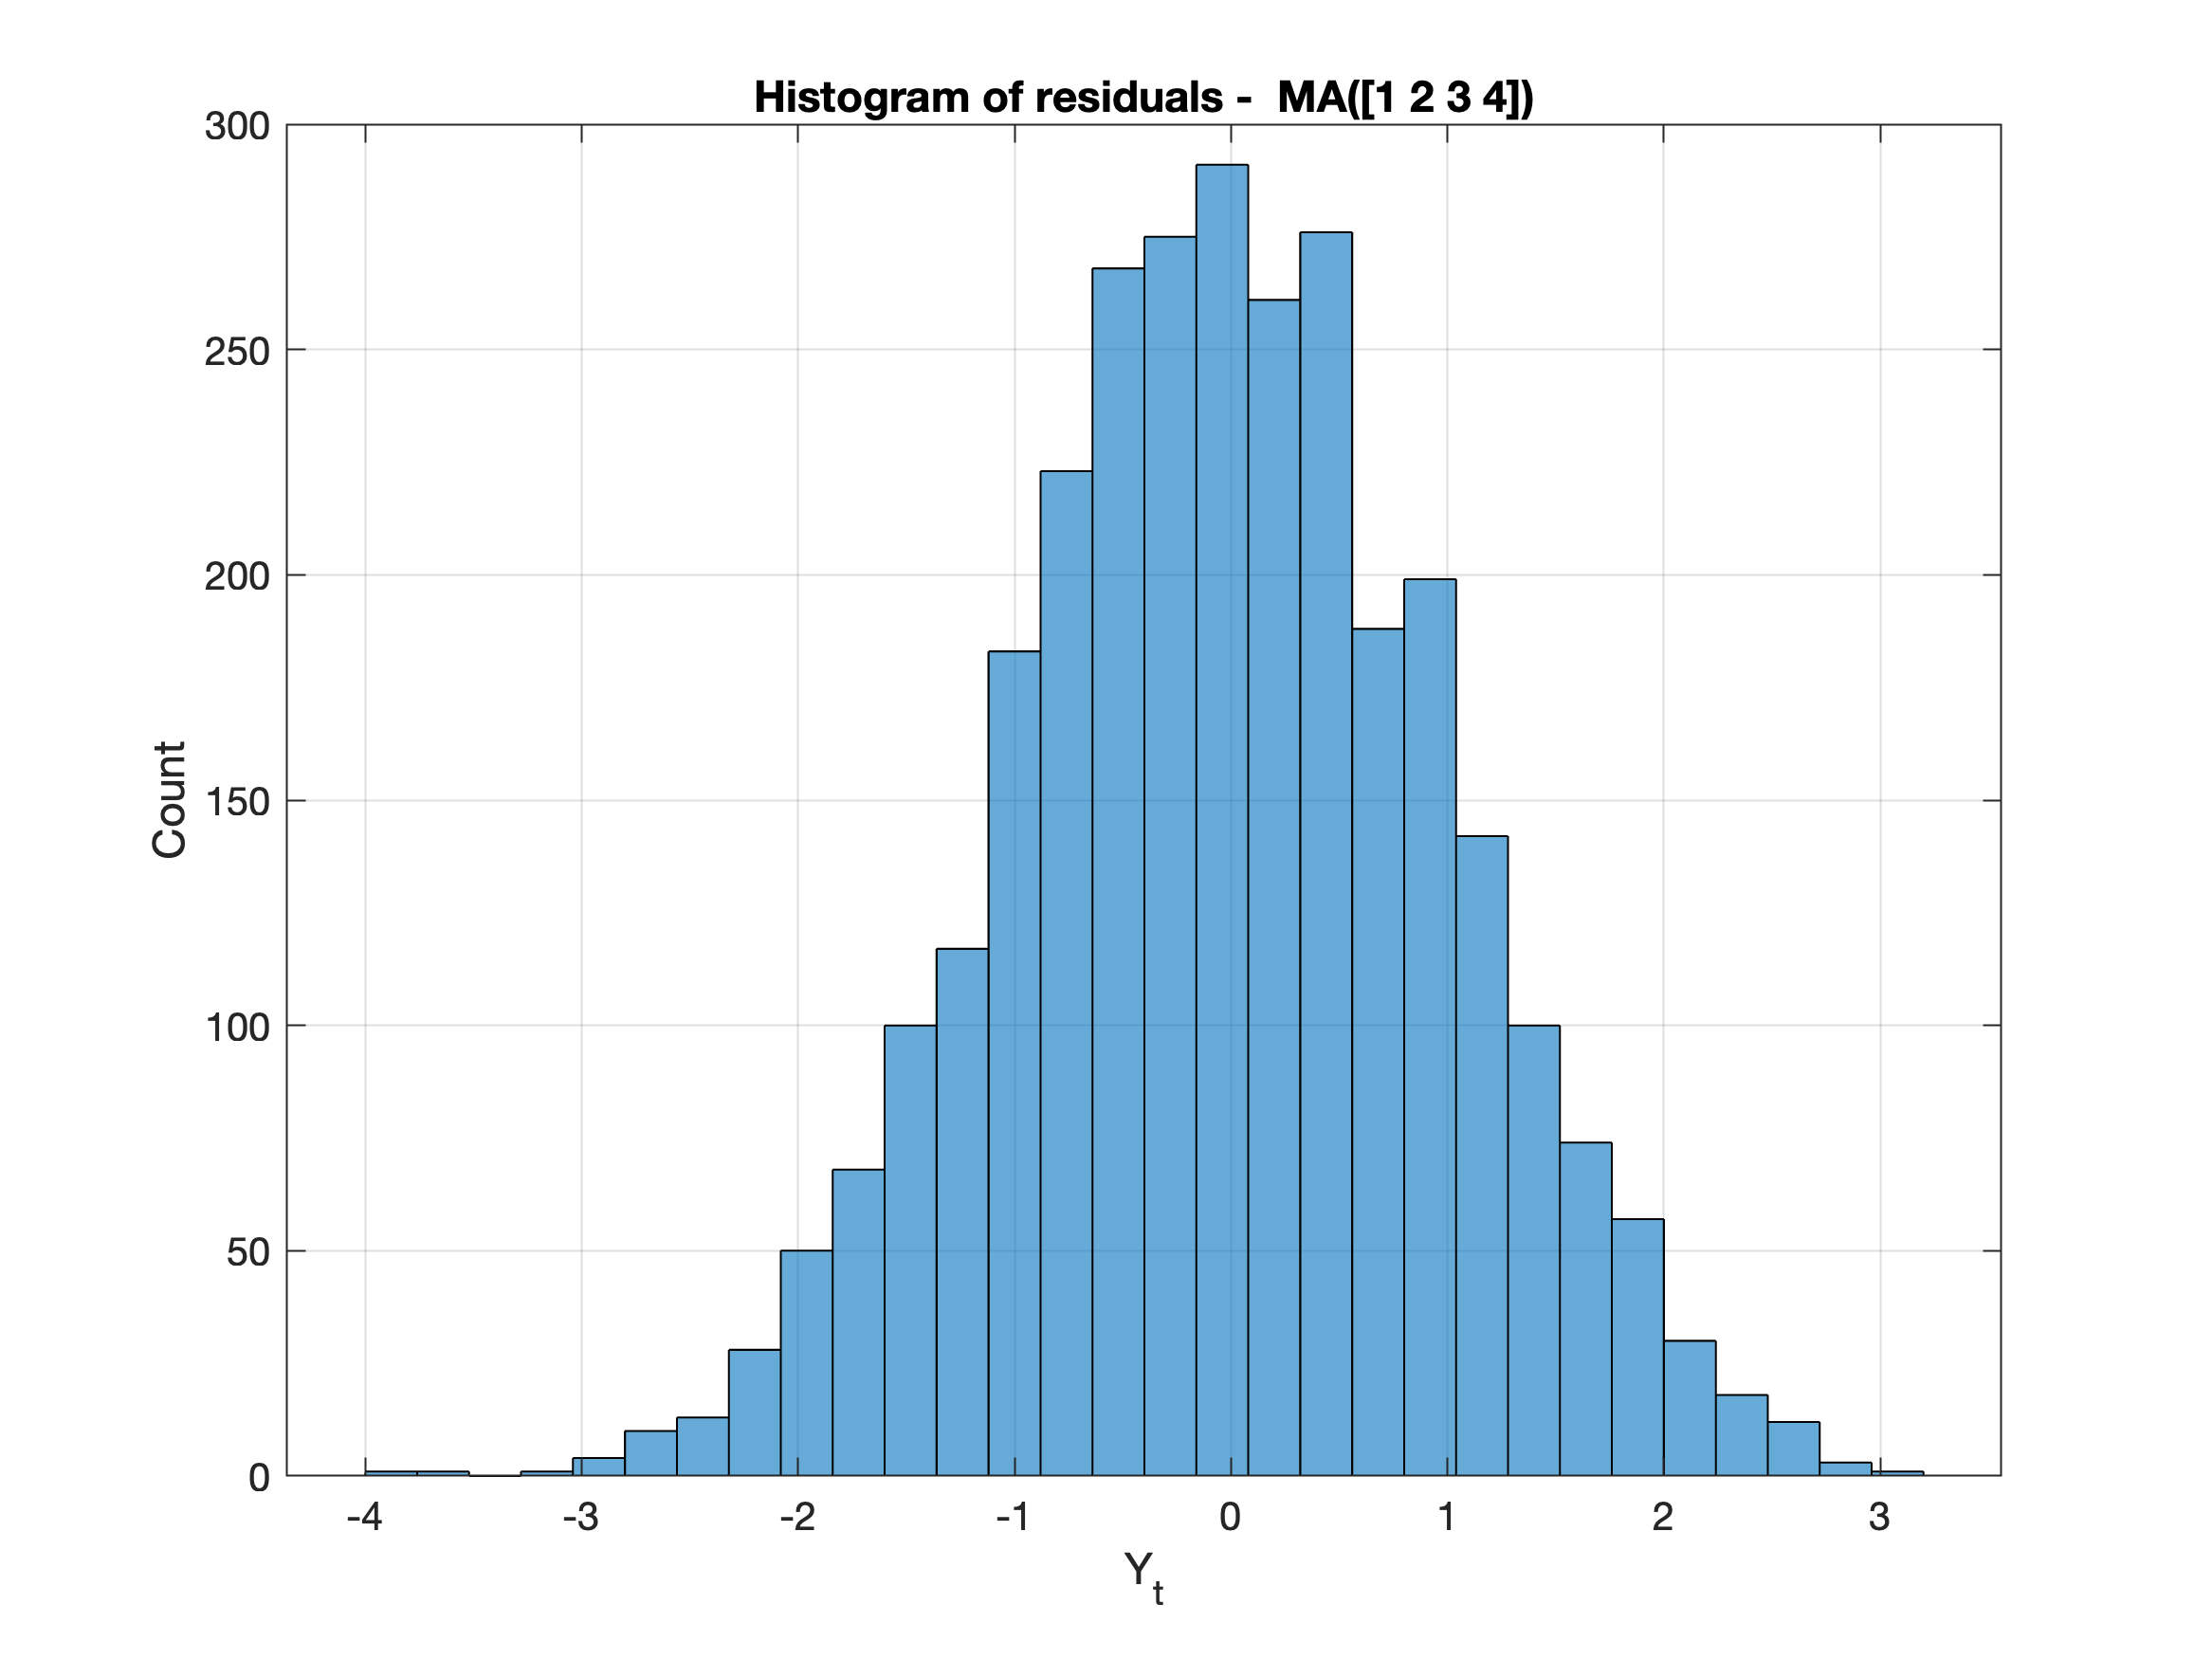
\includegraphics[width=\textwidth]{stationarity/step3c_resid_hist_MA.png}
    \caption{Histogram of residuals.}
    \label{fig:residuals-hist}
  \end{subfigure}\hfill
  \begin{subfigure}[t]{.49\textwidth}
    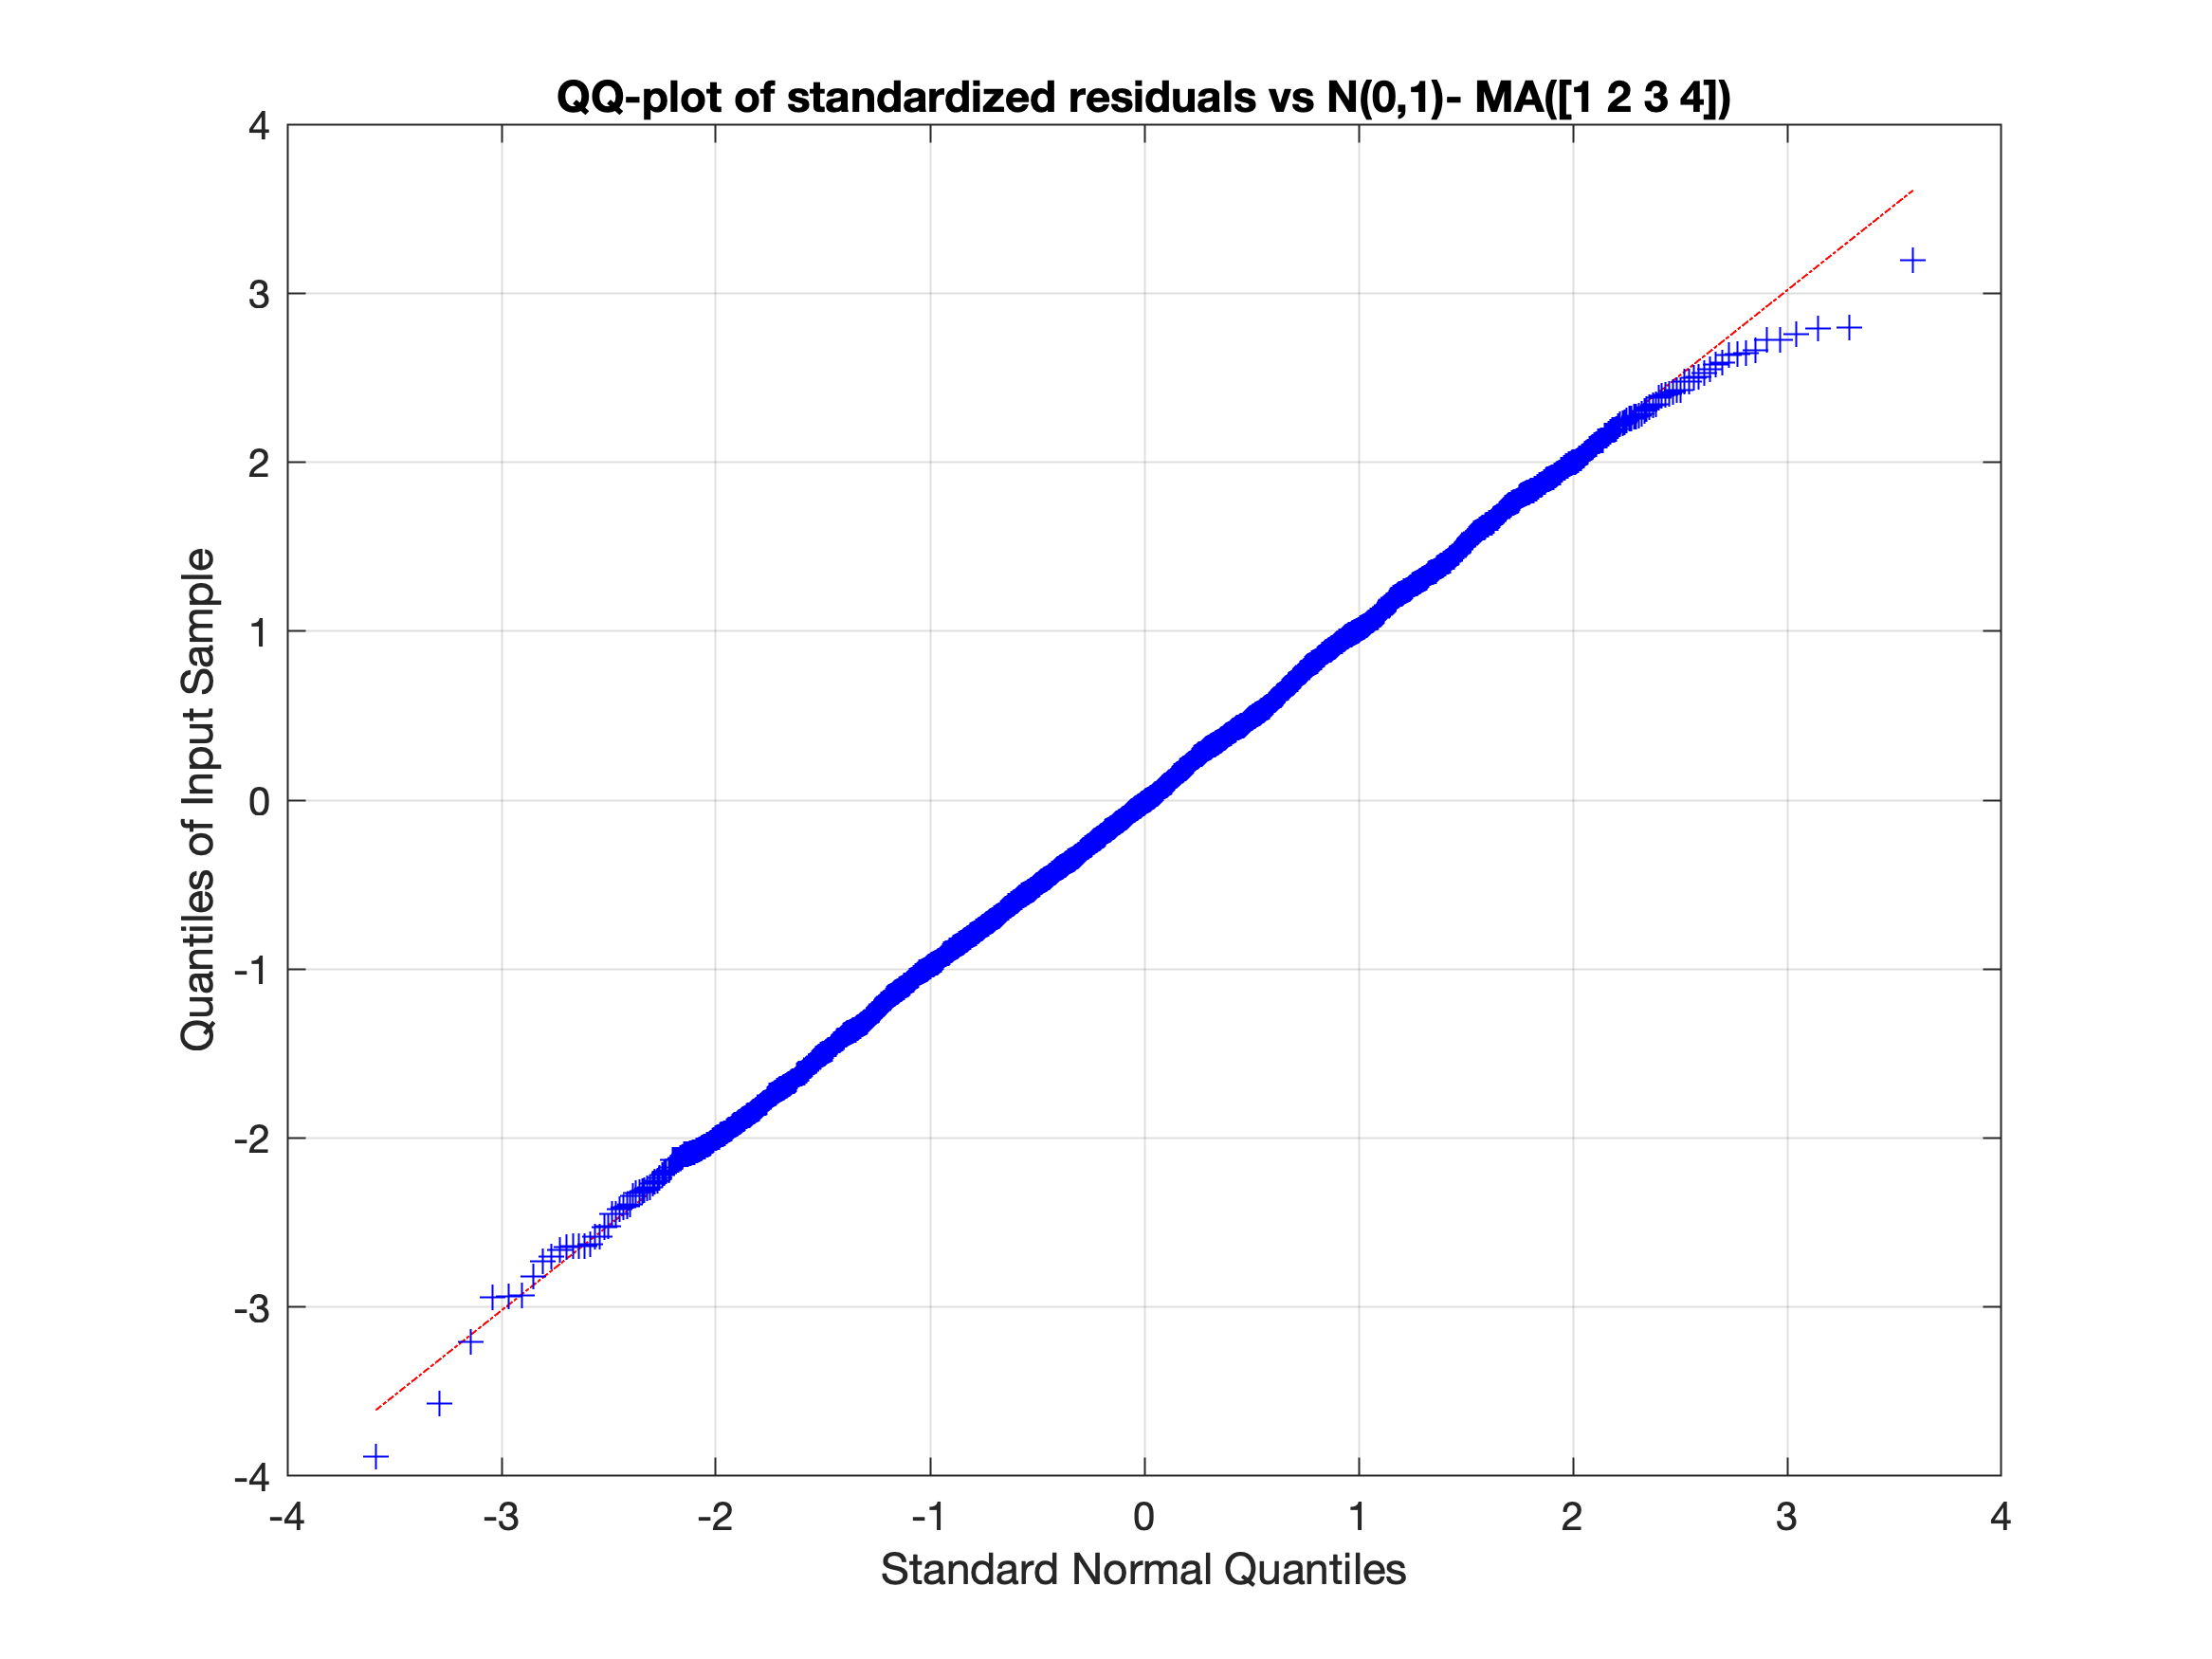
\includegraphics[width=\textwidth]{stationarity/step3c_resid_qqplot_MA.png}
    \caption{QQ-plot (standardized residuals vs.\ $N(0,1)$).}
    \label{fig:residuals-qq}
  \end{subfigure}
  \caption{Normality checks for residuals.}
  \label{fig:residuals-hist-qq}
\end{figure}

To test for ARCH effects, we inspect the SACF and SPACF of squared residuals (Figure~\ref{fig:yt-ma-resid2-acf-pacf}) and compute Ljung-Box tests on those. All resulting $p$-values lie above $0.79$ (up to lag~30), meaning that we find no evidence of conditional heteroscedasticity.

\begin{figure}[H]
  \centering
  \begin{subfigure}[t]{.49\textwidth}
    
\includegraphics[width=\textwidth]{stationarity/step3c_resid2_sacf_MA.png}
    \caption{SACF of squared $\mathrm{MA}(1,2,3,4)$ residuals.}
  \end{subfigure}\hfill
  \begin{subfigure}[t]{.49\textwidth}
    
\includegraphics[width=\textwidth]{stationarity/step3c_resid2_spacf_MA.png}
    \caption{SPACF of squared $\mathrm{MA}(1,2,3,4)$ residuals.}
  \end{subfigure}
  \caption{Dependence diagnostics for squared $\mathrm{MA}(1,2,3,4)$ residuals.}
  \label{fig:yt-ma-resid2-acf-pacf}
\end{figure}

All modeling assumptions are fulfilled: stationarity, invertibility, residuals exhibit no remaining linear dependence, approximate normality, and no ARCH effects. The $\mathrm{MA}(1,2,3,4)$ model without constant (insignificant, $Y_t$ is already centered around zero, see Figure~\ref{fig:residuals-hist}) is therefore our final stationary model for $Y_t$:
\[
Y_t
= a_t 
- 0.5929\,a_{t-1}
- 0.0837\,a_{t-2}
- 0.0651\,a_{t-3}
- 0.0856\,a_{t-4},
\]

\section{Predictions}

\begin{questionbox}
    Provide predictions for horizon $h = 1$ and try to evaluate how your predictions are correct.
\end{questionbox}

To evaluate the predictive power of our final stationary model $Y_t$ described in the previous section (Section~\ref{stationarity_section}), we perform a one-step-ahead forecasting exercise using the theory of MA models and a rolling origin approach. An MA model is a finite-memory process: its 1-step forecast depends on a finite number of past shocks, and multi-step forecasts converge rapidly to the unconditional mean.

\subsection{Predictions for horizon $h = 1$}

We split the available dataset of $T=2994$ observations into a training set containing the first $N_{train}=2974$ observations and a test set containing the last $N_{test}=20$ observations. Then, we follow the procedure below:

\begin{enumerate}
    \item \textbf{Parameter Re-estimation:} We re-estimate the identified $\mathrm{MA}(1,2,3,4)$ model using only the training data to prevent look-ahead bias. The re-estimated parameters yiels a residual standard deviation of $\hat{\sigma}_a = 0.9969$.
    \item \textbf{Forecasting (Stationary Scale):} For each time step $t$ in the test set, we compute the one-step-ahead forecast $\hat{r}_t(1)$ using the conditional expectation of the MA process:
    \[
        \hat{r}_t(1) = \hat{\mu} + \sum_{j \in \{1,2,3,4\}} \hat{\theta}_j a_{t-j}
    \]
    where $\hat{\mu}$ is the estimated constant (= mean of the series for MA models $= 0$ in our case) of the stationary series, and $\hat{\theta}_j$ are the estimated MA coefficients. Note that we use a '$+$' sign for the MA terms to match the convention of the \textit{armaxfilter} function (MFE Toolbox) used for estimation, which differs from the '$-$' sign convention found in the course syllabus. The term $a_{t-j}$ represents the past shock/innovation observed at time $t-j$, which is obtained recursively as the difference between the actual observed value and the forecast made at that time:
    \[
        a_{t-j} = r_{t-j} - \hat{r}_{t-j-1}(1) = e_{t-j}(1)
    \]
    This recursive calculation ensures that the information set $F_t$ is updated with the most recent prediction errors before forecasting the next step.
    \item \textbf{Reconstruction (Original Scale):} To generate forecasts for the original price series $X_t$, we invert the differencing operations (trend order $d=2$, seasonality $S=4$) using the filter polynomial $P(L) = (1-L^4)(1-L)^2$. The derivation for the reconstructed series $X_t$ is as follows: we define the stationary series $r_t$ as the result of applying the differencing polynomial $P(L)$ to the original series $X_t$:
    \[
        r_t = P(L) X_t
    \]
    Expanding the polynomial $P(L)$ yields:
    \[
        P(L) = 1 + \psi_1 L + \psi_2 L^2 + \dots + \psi_k L^k
    \]
    Substituting this expansion back into the definition of $r_t$:
    \begin{align}
        r_t &= (1 + \psi_1 L + \psi_2 L^2 + \dots + \psi_k L^k) X_t \\
        r_t &= X_t + \psi_1 X_{t-1} + \psi_2 X_{t-2} + \dots + \psi_k X_{t-k} \\
        r_t &= X_t + \sum_{j=1}^k \psi_j X_{t-j}
    \end{align}
    Solving for $X_t$, we obtain the general reconstruction formula:
    \[
        X_t = r_t - \sum_{j=1}^{k} \psi_j X_{t-j}
    \]
    Consequently, to reconstruct the one-step-ahead prediction $\hat{X}_t$, we use the forecasted stationary value $\hat{r}_{t-1}(1)$ and the known past values of $X$:
    \[
        \hat{X}_t = \hat{r}_{t-1}(1) - \sum_{j=1}^{k} \psi_j X_{t-j}
    \]
    where $k=6$ is the degree of the polynomial $P(L)$, and $\psi_j$ are the coefficients of the expanded polynomial $P(L)$. % (excluding the intercept)
\end{enumerate}

\subsection{Predictions evaluation}

We evaluate the accuracy of the predictions using the Root Mean Squared Error (RMSE) and we find that our series achieve a a score of $RMSE=1.09999$. This is is very close to the residual standard deviation estimated on the training set ($\hat{\sigma}_a \approx 0.9969$). This indicates that the model generalizes well and is not suffering from overfitting.\\ 

Visual inspection (Figure~\ref{fig:forecasts}) confirms that the model tracks the dynamics of the actual series closely. Regarding the uncertainty quantification, we observe that 2 out of the 20 test observations (10\%) fall slightly outside the 95\% confidence bands in Figure~\ref{fig:forecasts-stationary}. While this exceeds the theoretical expectation of 5\% (which would correspond to 1 point), it remains within an acceptable range for a small test sample, validating the overall adequacy of the $\mathrm{MA}(1,2,3,4)$ model for one-step-ahead forecasting.

\begin{figure}[H]
  \centering
  \begin{subfigure}[t]{.49\textwidth}
    
\includegraphics[width=\textwidth]{forecast/step4e_forecast.png}
    \caption{One-step-ahead forecasts for the stationary series.}
    \label{fig:forecasts-stationary}
  \end{subfigure}\hfill
  \begin{subfigure}[t]{.49\textwidth}
    
\includegraphics[width=\textwidth]{forecast/step4f_forecast_original_scale.png}
    \caption{One-step-ahead forecasts for the original series.}
    \label{fig:forecasts-original}
  \end{subfigure}
  \caption{One-step-ahead forecasts visualization.}
  \label{fig:forecasts}
\end{figure}

% %%%%%%%%%%%%%%%%%%%%%%%%%%%%%%%%%%%%%%%%%%%%%%%%%%%%%%%

%% Si besoin d'annexes
% \newpage
% \lhead{APPENDICES}
% \chapter*{Appendices}
% \addcontentsline{toc}{chapter}{Appendices} 
% Blabla

% %%%%%%%%%%%%%%%%%%%%%%%%%%%%%%%%%%%%%%%%%%%%%%%%%%%%%%%

\newpage
\printindex[Tot]

% %%%%%%%%%%%%%%%%%%%%%%%%%%%%%%%%%%%%%%%%%%%%%%%%%%%%%%%

% \newpage
% % \lhead{BIBLIOGRAPHY}
% % \rhead{}
% % \addcontentsline{toc}{chapter}{Bibliography}
% \bibliographystyle{unsrt-fr} 
% \bibliography{BibtexFileName}

% %%%%%%%%%%%%%%%%%%%%%%%%%%%%%%%%%%%%%%%%%%%%%%%%%%%%%%%

\end{document}


